\documentclass{ctexart}
\usepackage{amsmath}
\usepackage{amssymb}
\usepackage{graphicx}
\usepackage{geometry}
\usepackage{tikz}
\usepackage{pgfplots}
\usepackage{draftwatermark}

\geometry{a4paper, margin=2cm}
\pgfplotsset{compat=1.18}

% 添加专属学习资料水印
\SetWatermarkText{贺昱琪学习资料}
\SetWatermarkLightness{0.92}
\SetWatermarkScale{0.6}

\begin{document}

\title{贺昱琪核心错题精讲及针对性巩固}

\date{}
\maketitle

\section*{一、 规律探究与新定义}

\begin{enumerate}
    \item \textbf{先找大方向的规律（比如每行或每列的递增趋势、总个数），再结合坐标或拐点位置进行定位，不要盲目去数。}
    
    如图，图中的数字是从1开始按箭头方向排列的有序数阵，从3开始，把位于同一列且在拐角处的两个数字提取出来组成有序数对：(3,5), (7,10), (13,17), (21,26), (31,37)……，则第19个数对是 \underline{\hspace{2cm}}。
    \hfill
    \begin{minipage}{0.3\textwidth}
        \centering
        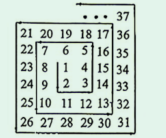
\includegraphics[width=\linewidth]{1.png}
    \end{minipage}
    \vspace{2cm}

    \item \textbf{紧扣题目的“新定义”，把文字条件转化为代数式。利用整除的特征（能被10整除说明个位是0），结合数字0-9的范围限制进行枚举或放缩。}
    
    对于一个四位自然数M，若它的千位数字比个位数字多6，百位数字比十位数字多2，则称为“天真数”，如：四位数7311，因为$7-1=6$，$3-1=2$，所以7311是“天真数”；因为$8-1\neq6$，所以8421不是“天真数”。一个“天真数”M的千位数字为a，百位数字为b，十位数字为c，个位数字为d，记 $P(M)=3(a+b)+c+d$，$Q(M)=a-5$，若 $\frac{P(M)}{Q(M)}$ 能被10整除，则满足条件的M的最大值为 \underline{\hspace{2cm}}。
    \vspace{2cm}

    \item \textbf{明确间隔条件，设出未知数后有条理地列举。注意这里的边界条件，琴键总数不超过12，做到不重不漏。}
    
    将钢琴上的12个键依次记为 $a_1, a_2, \dots, a_{12}$。设 $1\le i<j<k\le 12$。若 $k-j=3$ 且 $j-i=4$，则称原位大三和弦；若 $k-j=4$ 且 $j-i=3$，则称原位小三和弦。构成的原位大三和弦与原位小三和弦的个数之和为 \underline{\hspace{2cm}}。
    \vspace{2cm}
    
    \item \textbf{利用平方差公式 $(a+b)(a-b)$ 逆向拆分。注意奇偶性分析，奇数、4的倍数、4k+2型数的拆分情况是不同的，分类找规律。}
    
    如果一个正整数能表示为两个正整数的平方差，那么称这个正整数为“智慧数”。
    (1) 请将第8个智慧数仿照小颖的方法写出来 \underline{\hspace{2cm}}；
    (2) 800这个智慧数可分解为 \underline{\hspace{2cm}} 和 \underline{\hspace{2cm}} 的平方差；
    (3) 判断形如 $4k+2$ ($k$为正整数) 的数 \underline{\hspace{2cm}} 智慧数（填是或不是）；
    (4) 请求出第2025个智慧数的值。
    \vspace{2cm}
\end{enumerate}

\section*{二、 应用题与代数综合}

\begin{enumerate}
    \item \textbf{设燃尽时间，根据“剩余长度 = 原长 - 燃烧速度$\times$时间”来建立等量关系。}
    
    有两支蜡烛一样长，第一支5小时燃尽，第二支3小时燃尽，如果同时点燃这两支蜡烛，且蜡烛燃烧的速度不变，在点燃几小时后，第一支蜡烛的长度是第二支蜡烛的3倍？
    \vspace{2cm}

    \item \textbf{抓住隐含的等量关系：总售价 - 总进价 = 总利润。重点注意“还剩5双”，意味着进货量比售出量多了5。}
    
    超市以每双8.5元的价格购进一批拖鞋，销售价为10.4元，卖到还剩5双时，除成本外还获利147.5元，这批拖鞋已经卖出多少双？
    \vspace{2cm}

    \item \textbf{认真读表格，分段计费。重点理清申请前和申请后阶梯临界点的变化，分别算出总价再求差。}
    
    为增强公民的节约意识，合理利用水资源，我市发改委对市城区公共管网全年供水量实行阶梯式水价，其中，居民全年阶梯水量按每户4口人计，居民家庭人口超过4人的，每增加1人，可申请在各阶梯年度水量基础上增加36$m^3$。若小明家现有5口人，全年用水量为160$m^3$，则申请前比申请后全年多缴费多少元？
    \vspace{2cm}

    \item \textbf{一定要画线段图辅助！两次改变速度，对应两次新的相遇过程。抓准整个过程不变的量（总路程不变）列方程组。}
    
    甲、乙两车分别从A、B两地同时出发相向而行，6小时后相遇在C地。如果甲车的速度不变，乙车每小时多行5千米，且两车还从A、B两地同时出发相向而行，则相遇的地点距离C地12千米；如果乙车的速度不变，甲车每小时多行5千米，且两车还从A、B两地同时出发相向而行，则相遇地点距离C地16千米。求甲车原来每小时行多少千米？
    \vspace{2cm}

    \item \textbf{遇到方案优选，直接设出两次的具体油价 $a$ 和 $b$。分别列出平均单价的代数式，用作差法或者基本不等式比大小。}
    
    汽油的单价会随着各种因素不断变动，一段时间内，某人计划去加油站加两次油，现有两种加油方案；甲方案：每次加油的总金额固定；乙方案：每次所加的油量固定。规定平均单价越低越实惠，不考虑其他因素影响，则以下四种方案中（①甲方案实惠；②乙方案实惠；③需由两次油价决定；④一样实惠），你认同的是 \underline{\hspace{2cm}}。
    \vspace{2cm}

    \item \textbf{设出未知数，找准“取出前”和“取出后”早晚粮食分配的比例变化关系，列出一元一次方程。}
    
    成语“朝三暮四”讲述老翁分早晚两次喂食猴群。老翁从晚上的粮食中取出2千克放在早上投食，这样早上的粮食是晚上的 $\frac{4}{3}$，猴群欣然接受。求老翁给猴群每日的供应量是多少千克？
    \vspace{2cm}

    \item \textbf{相遇问题中，路程比 = 速度比 $\times$ 时间比。千万注意甲晚出发的这个条件对双方实际行驶时间的影响。}
    
    甲、乙两车相向而行，乙车的速度是甲车的 $\frac{4}{5}$，乙车先出发开往A地，出发48千米后，甲车从A地出发。两车相遇时的地方离A、B两地距离比是3:4，A、B两地相距多少千米？
    \vspace{2cm}
    
    \item \textbf{连续自然数求和公式配合平均数。由平均数 $53\frac{3}{7}$ 先推断出总个数 $n$ （大概在106左右），再利用总和守恒求被删去的数字。}
    
    将若干由1开始的连续自然数写在纸上，然后删去其中一个数，则余下的数的平均数为 $53\frac{3}{7}$，问删去的那个数是 \underline{\hspace{2cm}}。
    \vspace{2cm}
\end{enumerate}

\section*{三、 几何图形与动点问题}

\begin{enumerate}
    \item \textbf{利用全等三角形进行面积割补，不论三角板怎么旋转，重叠部分的面积往往恒等于正方形面积的四分之一。}
    
    某兴趣小组在一次综合与实践活动中提出这样一个问题：将足够大的直角三角板PEF ($\angle P=90^\circ, \angle F=60^\circ$) 的一个顶点放在正方形ABCD中心O处，并绕点O顺时针旋转，探究直角三角板PEF与正方形ABCD重叠部分的面积变化情况（已知正方形边长为2）。
    (1) 若将三角板的顶点P放在点O处，在旋转过程中，当OF与OB重合时，重叠部分的面积为 \underline{\hspace{2cm}}；当OF与AB垂直时，重叠部分的面积为 \underline{\hspace{2cm}}。一般地，若正方形面积为a，在旋转过程中，重叠部分的面积S与a的关系为 \underline{\hspace{2cm}}。
    (2) 将该三角板的顶点F放在等边三角形ABC的中心O处，边OE经过点B。将该三角板绕点O顺时针旋转$\alpha$ ($0^\circ\le\alpha\le120^\circ$)，在旋转过程中，重叠部分的面积如何变化？
    \hfill
    \begin{minipage}{0.3\textwidth}
        \centering
        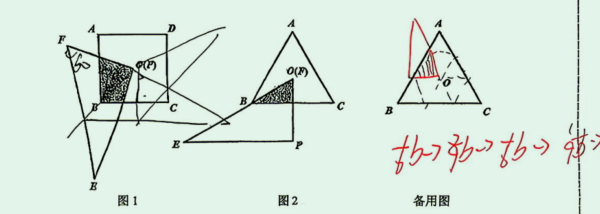
\includegraphics[width=\linewidth]{2.png}
    \end{minipage}
    \vspace{2cm}

    \item \textbf{折叠的本质就是轴对称。抓住折叠前后的对应角相等，再利用平角 $180^\circ$ 倒推。}
    
    如图，在长方形纸片ABCD中，点P是BC边上一点，沿着AP折叠纸片并展开，点B落在B'处，当AB'与AD边的夹角为 $15^\circ$ 时，$\angle APB$ 的度数是 \underline{\hspace{2cm}}。
    \hfill
    \begin{minipage}{0.3\textwidth}
        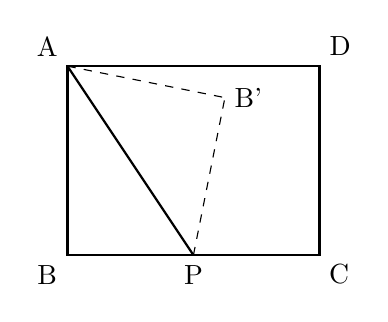
\begin{tikzpicture}[scale=0.8]
            \draw[thick] (0,0) node[below left]{B} rectangle (4,3) node[above right]{D};
            \node[above left] at (0,3) {A};
            \node[below right] at (4,0) {C};
            \coordinate (P) at (2,0);
            \draw[thick] (0,3) -- (P) node[below]{P};
            \coordinate (Bprime) at (2.5, 2.5);
            \draw[dashed] (0,3) -- (Bprime) node[right]{B'};
            \draw[dashed] (P) -- (Bprime);
        \end{tikzpicture}
    \end{minipage}
    \vspace{2cm}

    \item \textbf{灵活利用 $S_{\triangle} = \frac{1}{2} S_{平行四边形}$ 的等底等高性质，通过面积的加减容斥来求解。}
    
    如图，平行四边形ABCD中，若 $\triangle BGE$ 的面积为2，$\triangle PDF$ 的面积为3，四边形CEHF的面积为18，则阴影部分四边形AGHP的面积为 \underline{\hspace{2cm}}。
    \hfill
    \begin{minipage}{0.3\textwidth}
        \centering
        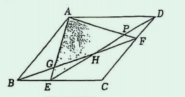
\includegraphics[width=\linewidth]{3.png}
    \end{minipage}
    \vspace{2cm}

    \item \textbf{选好基准量（比如设胸腹高为 $x$），把其他所有线段都用含 $x$ 的式子表达出来，最后找等量关系解方程。}
    
    为制作一只风筝，小明准备了一根门条、两根膀条和两根尾条。头部高、胸腹高与尾部高的比是1:1:2。已知单根膀条长是胸腹高的5倍，门条比单根膀条短10cm，BC的长是门条长的 $\frac{5}{9}$，AB、CD的长均等于胸腹高。求这只风筝的骨架的总高。
    \hfill
    \begin{minipage}{0.3\textwidth}
        \centering
        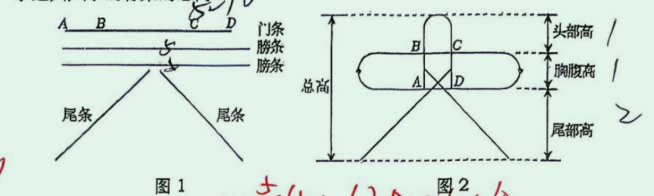
\includegraphics[width=\linewidth]{4.png}
    \end{minipage}
    \vspace{2cm}

    \item \textbf{容斥原理的典型应用：总长 = 甲长 + 乙长 - 重叠长。代入题目的比例算即可。}
    
    甲、乙两张等宽的长方形纸条，长分别为a，b。将甲纸条的 $\frac{1}{3}$ 与乙纸条的 $\frac{2}{5}$ 叠合在一起，形成长为81的纸条，则 $a+b=$ \underline{\hspace{2cm}}。
    \vspace{2cm}

    \item \textbf{利用面积公式 $ah_a = bh_b = ch_c$ 将高的关系转化为边长的比例，再结合三角形三边关系（两边之差<第三边<两边之和）卡出范围。}
    
    已知 $\triangle ABC$ 的两条高线的长分别为5和20，若第三条高线的长也是整数，则第三条高线长的最大值为 \underline{\hspace{2cm}}。
    \vspace{2cm}

    \item \textbf{数形结合，将右侧函数图象的拐点转折时间，跟左侧动点在长方形顶点上的位置一一对应，分段解出速度和各边边长。}
    
    如图，长方形ABCD中，点P沿着四边按 $B\to C\to D\to A$ 方向运动，点P运动到点A时停止运动。开始以每秒m个单位匀速运动，a秒后变为每秒2个单位匀速运动，b秒后恢复原速匀速运动，在运动过程中，$\triangle ABP$ 的面积S与运动时间t之间的关系如下图所示。
    (1) 长方形ABCD的长BC= \underline{\hspace{2cm}}，宽CD= \underline{\hspace{2cm}}；
    (2) m= \underline{\hspace{2cm}}，a= \underline{\hspace{2cm}}，b= \underline{\hspace{2cm}}；
    (3) 当S=10时，则运动的时间t= \underline{\hspace{2cm}}。
    \hfill
    \begin{minipage}{0.3\textwidth}
        \centering
        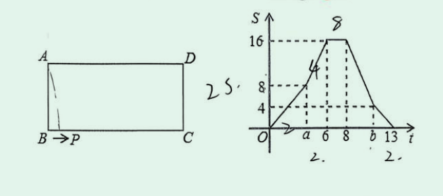
\includegraphics[width=\linewidth]{5.png}
    \end{minipage}
    \vspace{2cm}
\end{enumerate}

\newpage
\section*{其他错题梳理}

\subsection*{第一类：基础计算与代数式}
\begin{enumerate}
    \item \textbf{注意 $3.0$ 的精确度到十分位，范围卡紧上下限。} \\
    近似数 3.0的取值范围是 \underline{\hspace{2cm}}。
    \vspace{2cm}
    \vspace{2cm}
    
    \item \textbf{看到复杂的带分数加减，先把整数部分和分数部分拆开分别算，灵活变通。} \\
    计算：$2\frac{5}{6}-3\frac{1}{12}+4\frac{19}{20}-5\frac{1}{30}+6\frac{41}{42}-1\frac{1}{2}$
    \vspace{2cm}
    \vspace{2cm}
    
    \item \textbf{算式太长肯定有巧算，寻找相同的因数或倍数提出来化简。} \\
    计算：$(7.5\times9.9+75\times0.16-750\times0.015)\div\left(\frac{1}{2}-\frac{1}{3}\right)\times6$ 
    \vspace{2cm}
    \vspace{2cm}
    \item \textbf{理清原价、标价、售价的换算关系，设未知数直接求解。} \\
    一件商品按标价打六折出售，仍可获利20\%，已知这件商品的进价是100元，则标价为 \underline{\hspace{2cm}} 元。
    \vspace{2cm}
    \vspace{2cm}
    \item \textbf{要凑完全平方数，就把 7920 分解质因数，看哪个质因数的指数是奇数，补齐它就行。} \\
    一个非零整数a与7920的积是一个完全平方数，则a的最小值为 \underline{\hspace{2cm}}。
    \vspace{2cm}
    \vspace{2cm}
    \item \textbf{观察分子和分母的联系，这很可能是一个斐波那契数列的变形。} \\
    下面是一串有规律的数：$1, \frac{3}{2}, \frac{8}{5}, \frac{21}{13}, \frac{55}{34}, \dots$ 从左至右，这串数中的第7个数是 \underline{\hspace{2cm}}。
    \vspace{2cm}
    \vspace{2cm}
\end{enumerate}

\subsection*{第二类：几何图形进阶}
\begin{enumerate}
    \item \textbf{利用对称性，把阴影部分割补拼凑成规则的半圆或扇形。} \\
    画出了一个大圆和四个面积相等的小圆，已知大圆半径等于小圆直径，小圆面积为8平方厘米，那么阴影部分的面积总和为 \underline{\hspace{2cm}} 平方厘米。
    \vspace{2cm}
    \vspace{2cm}
    \item \textbf{遇到多条线段被按比例截断，利用等高三角形的面积比等于底边比一步步向内推。} \\
    在 $\triangle ABC$ 中，$BD=2AD$，$AG=2CG$，$BE=EF=FC=\frac{1}{3}BC$，求特定小三角形面积占比。
    \vspace{2cm}
    \vspace{2cm}
    \item \textbf{旋转扫过的区域本质上是圆环的一部分或扇形，套用公式含 $\pi$ 计算即可。} \\
    直角三角形绕B点旋转120°，求扫过阴影部分面积（含 $\pi$ 计算）。
    \vspace{2cm}
    \vspace{2cm}
    \item \textbf{遇到一连串的中点，利用相似比或者构建坐标系求交点算面积都很直接。} \\
    如图，已知边长为8的正方形ABCD，E为AD的中点，P为CE的中点，则 $\triangle BDP$ 的面积是 \underline{\hspace{2cm}}。
    \vspace{2cm}
    \vspace{2cm}
    \item \textbf{正放液体的体积不变，倒放时空着的部分体积就等于瓶子总体积减去液体体积，两头一凑就出来了。} \\
    有一种饮料瓶的瓶身呈圆柱形，瓶子的容积为400立方厘米。正放时，液体高20厘米，倒放时空余部分高5厘米，则瓶内饮料的体积为 \underline{\hspace{2cm}} 立方厘米。
    \vspace{2cm}
    \vspace{2cm}
    \item \textbf{反复折叠重合说明角被平分，找出外角和内角的数量关系列方程。} \\
    探究：沿 $\triangle ABC$ 的 $\angle BAC$ 的平分线折叠，只要最后一次恰好重合称为“好角”，寻找底角之间的倍数关系。
    \vspace{2cm}
    \vspace{2cm}
\end{enumerate}

\subsection*{第三类：综合推理与应用题}
\begin{enumerate}
    \item \textbf{从 $n=1,2,3$ 慢慢画，列个表格找规律，看每次增加的点是怎么把原有的三角形一分为三的。} \\
    $\triangle ABC$ 内部1个点连线分出3个三角形，2个点分出5个...探究 $n$ 个点可分出几个小三角形。
    \vspace{2cm}
    \vspace{2cm}
    \item \textbf{画好各阶段时间轴，注意“停留时间”和双方的速度差。} \\
    小强骑车游玩，停留后返回，妈妈驾车迎接，已知小强骑车的速度为15千米/时，妈妈驾车的速度为60千米/时，根据多段运动时间差求相遇时间。
    \vspace{2cm}
    \vspace{2cm}
    \item \textbf{设规定时间为 $x$，把工作总量看作1，列出甲乙各自的效率表达式。} \\
    单独完成一项工作，甲按规定时间可提前2天完成，乙则要超过规定时间3天才能完成。如果甲、乙二人合做两天后，剩下的由乙单独做，那么刚好在规定时间完成。求合做需多少天。
    \vspace{2cm}
    \vspace{2cm}
    \item \textbf{原价设为 $x$，列出变化后的成本和售价，利润 = 售价 - 成本。} \\
    某房地产开发商开发一套房子的成本随着物价上涨比原来增加了10\%，为了赚钱，开发商把售价提高了0.5倍，利润率比原来增加了60\%，求开发商原来的利润率。
    \vspace{2cm}
    \vspace{2cm}
    \item \textbf{信息量大时一定要列出各个相遇时间点的距离表达式，逐步削减未知量。} \\
    在一条公路上汽车A、B、C分别以每小时80、60、40千米的速度行驶，汽车A从甲站开往乙站，同时汽车B、C从乙站出发与A相向而行，途中车A与车B相遇后两小时再与车C相遇，求甲乙两站距离。
    \vspace{2cm}
    \vspace{2cm}
\end{enumerate}

\end{document}